\section{Планирование траекторий движения манипулятора}\label{part_trajectory}
%%% http://www-lar.deis.unibo.it/people/cmelchiorri/foundations_robotics.html

Рассматриваются задачи планирования траекторий движения манипулятора в  решении комплексных задач: перемещению в рабочем пространстве и взаимодействию с целевыми объектами.

\subsection{Постановка и описание задачи}

Успешность захвата манипулятором, перемещающегося по конвейеру объекта заключается, как в качественной работе системы управления манипулятором, так и в планировании траектории движения его схвата, которая в точности должна повторять движение объекта.

Планирование траектории подразумевает получение программной зависимости перемещения звеньев манипулятора $ \mathbf{q}(t) $ или схвата $ \mathbf{s}(t) $ на интервале $ t \in [t_s, t_f] $. Тут $ \mathbf{q} = [q_1, q_2, \dots, q_n]^T$~--- вектор обобщенных координат, $ \mathbf{s} = [x,y,z, \varphi, \psi, \theta]^T $~--- вектор положения схвата относительно базовой СК $ Ox_0y_0z_0 $.

Необходимо спланировать траектории в пространстве обобщенных координат: для задания необходимой конфигурации робота~--- удобная ориентации камеры, закрепленной на последнем звене манипулятора (перевод из точки в точку); для обхода последовательности точек~--- осознанное перемещения объекта в рабочем пространстве от конвейера в зону погрузки. Недостатком такого подхода является то, что такие траектории нельзя использовать в операциях, где задача движения формулируется в пространстве координат схвата.

Также, необходимо спланировать траекторию в пространстве координат схвата для выполнения захватывания движущегося по конвейеру объекта.

Очевидно, что манипулятор с количеством степеней свободы $ N < 6 $ ограничен в своих движениях и, как видно из рассмотренной ранее кинематики манипулятора KUKA YouBot, он не может занимать любые необходимые ориентации, из чего следует, что в задаче решаемой в этой работе конвейер необходимо располагать параллельно плоскости OXY СК $ Ox_{0}y_{0}z_{0} $.

Также заметим, что рабочая область манипулятора при схвате сориентированном перпендикулярно плоскости OXY СК $ Ox_{0}y_{0}z_{0} $ (или, что тоже самое, рабочей плоскости конвейера) существенно ограничена. На рисунке~\ref{img:work_space_noraml} зеленым выделена рабочая область, в которой возможен захват объектов с конвейера или любой другой плоскости, удовлетворяющих условию параллельности описанному выше.

%Далее рабочую область с рисунка~\ref{img:work_space_noraml} будем называть нормальной рабочей областью.

\begin{figure}[h!]
	\centering\includegraphics[width=0.8\textwidth]{ipe/ws.pdf}
	\vspace{0.5cm}
	\caption{Рабочая область манипулятора робота KUKA Youbot при ориентации схвата перпендикулярной плоскости OXY СК $ Ox_{0}y_{0}z_{0} $ с учетом ограничений по допустимым углам поворотов сочленений и зоной безопасности в виде цилиндра вокруг оси $ z_0 $ c радиусом R и высотой H}
	\label{img:work_space_noraml}
\end{figure}

Запишем последовательность действий, необходимую для захвата объекта с конвейера:
\begin{enumerate}
	\item привести манипулятор в положения для работы СТЗ;
	\item перевести манипулятор в точку пересечения траектории движения объекта по конвейеру с нормальной рабочей областью манипулятора (точка $ p_0 $ на рисунке~\ref{img:ws_and_conveyer.pdf});
	\item провести манипулятор по траектории, совпадающей с траекторией движения объекта по конвейеру~\footnote{Эта траектория представляет из себя кривую расположенную над движущимся объектом. Т.е. манипулятор следует за объектом на некотором расстоянии над ним, пока не выровняются их скорости, после чего схват опускается на высоту объекта, захватывает объект и поднимается на прежнее расcтояние.};
	\item захватить объект;
	\item перенести объект в зону для складывания объектов с конвейера.
\end{enumerate}

%%% добавить рисунок с линейным конвейером АААААА Я НЕ УСПЕЛ((9
\begin{figure}[h!]
	\centering\includegraphics[width=0.55\textwidth]{ipe/ws_and_conveyer.pdf}
	\vspace{0.5cm}
	\caption{Пересечение плоскости конвейра и рабочей области манипулятора}
	\label{img:ws_and_conveyer.pdf}
\end{figure}


\subsection{Распределение допустимых скоростей в рабочем пространстве}

Необходимо выбрать траекторию движения схвата манипулятора такую, чтобы законы изменения положения, скоростей и ускорения, с одной стороны, соответствовали параметрам движения конвейера, а с другой~--- возможностям манипулятора.

Ограничения по скоростям в сочленениях заданы константами $ C_i $:
\begin{equation}\label{constrs}
|\dot{q}| \le C_i, \quad i = \overline{1,n}.
\end{equation}

Соотношения~\eqref{constrs} задают область допустимых скоростей в пространстве обобщенных координат. Скорости схвата рассчитывается из соотношений~\eqref{Jv1}--\eqref{Jw1} для решения прямой задачи о скорости и определяют отображение области допустимых скоростей в сочленениях в трехмерную область допустимых скоростей $ \bm{v}_n $, которую можно найти для каждой точки рабочего пространства. Определяя такие отображения для заданных всех возможных вариантов вектора $ \bm{q} $ можно найти распределение допустимых скоростей схвата в рабочем пространстве.

В практической реализации ограничимся получением оценки снизу и сверху значений скорости $ \bm{v}_n $ в рабочей зоне. Для этого определим евклидову норму вектора скорости $ \bm{v}_n $:
\begin{equation}
||\bm{v}_n|| = (\bm{v}^T \cdot \bm{v})^{\frac{1}{2}} = (\dot{\bm{q}}^T \cdot J_v^T(\bm{q}) \cdot J_v(\bm{q}) \cdot  \dot{\bm{q}})^{\frac{1}{2}}
\end{equation}
Тогда, обозначив за минимальное $ \underline{\lambda}(q) $ и максимальное $ \overline{\lambda}(q) $ характеристические числа матрицы $  J_v^T(\bm{q}) \cdot J_v(\bm{q}) $ и на основании свойств квадратичных форм, запишем:
\begin{equation}
\underline{\lambda}(q) \cdot ||\dot{\bm{q}}||^2 \le || \bm{v}_n ||^2 \le \overline{\lambda}(q) \cdot ||\dot{\bm{q}}||^2,
\end{equation}

Окончательно, для ограничения скоростей движения схвата сверху, оценка имеет вид:
\begin{equation}
||\bm{v}_n(q)|| \le \sqrt{\overline{\lambda}(q)} \cdot ||\dot{\bm{q}}|| < \sqrt{\overline{\lambda}(q)} \cdot C,
\end{equation}
где $ C = \sqrt{\sum_{i=1}^{n} C_i^2(q)} $.

Полученная оценка не может быть найдена в вырожденных конфигурациях манипулятора, а также на границах рабочей области.


%%%%%%%%%%%%%%%%%%%%%%%%%%%%%%%%%%%%%%%%%%%%%
%%%%%%%%%%%%%%%%%%%%%%%%%%%%%%%%%%%%%%%%%%%%%
%%%%%%%%%%%%%%%%%%%%%%%%%%%%%%%%%%%%%%%%%%%%%
\subsection{Планирование траектории в пространстве обобщенных координат}

Рассмотрим движение манипулятора из точки в точку, затем расширим это решение на движение через заданную последовательность точек.


%%%%%%%%%%%%%%%%%%%%%%%%%%%%%%%%%%%%%%%%%%%%%
%%%%%%%%%%%%%%%%%%%%%%%%%%%%%%%%%%%%%%%%%%%%%
%%%%%%%%%%%%%%%%%%%%%%%%%%%%%%%%%%%%%%%%%%%%%
\vspace{0.5cm}
\subsubsection{Движение из точки в точку}

Движение манипулятора в пространстве обобщенных координат из точки~$ \mathbf{q}_s $ в~точку $ \mathbf{q}_f $ формулируется, как:
\begin{equation}
	\mathbf{q} = \mathbf{q}(t),\,\,t \in [t_s, t_f],
\end{equation}
при граничных условиях:
\begin{equation}
	\mathbf{q}(t_s) = \mathbf{q}_s, 
	\quad
	\mathbf{q}(t_f) = \mathbf{q}_f.
\end{equation}


Такое движение можно обеспечить используя кривую, составленную из парабол на участках разгона и торможения и прямой на участке с постоянной скоростью. Пример такой траектории изображен на рисунке~\ref{img:plp}.

\begin{figure}[h!]
	\centering\includegraphics[width=0.7\textwidth]{ipe/plp.pdf}
	\vspace{0.5cm}
	\caption{Траектория с постоянной скоростью на среднем участке}
	\label{img:plp}
\end{figure}

Введем ограничение максимальной скорости $ v = v_{des} $.
Тогда время отработки траектории из точки~$ \bm{q}_s $ в точку~$ \bm{q}_f $ можно записать:
\begin{equation}
	t_f = \cfrac{3}{2} \cdot \cfrac{\bm{q}_f - \bm{q}_s}{v}.
\end{equation}
Отсюда, время разгона (торможения) и границы ускорений:
\begin{equation}
	t_b = \cfrac{\bm{q}_s - \bm{q}_f + v * t_f}{v}, \quad a = \cfrac{v}{t_b}.
\end{equation}
Траектория раcчитывается из следующих соотношений:
\begin{align}
	\bm{q}(t) = 
	\begin{cases}
		\bm{q}_s + \cfrac{a}{2} \cdot t^2, &t_s \le t \le t_b, \\
		\bm{q}_s + \cfrac{a}{2} \cdot t^2, &t_b < t \le t_f - t_b,\\
		\bm{q}_s + \cfrac{a}{2} \cdot t^2, &t_f - t_b < t \le t_f.
	\end{cases}
\end{align}
Скорости получаем из:
\begin{align}
	\dot{\bm{q}}(t) = 
	\begin{cases}
		a  t, &t_s \le t \le t_b, \\
		v, &t_b < t \le t_f - t_b,\\
		a  t_f - a * t, &t_f - t_b < t \le t_f.
	\end{cases}
\end{align}
Ускорения:
\begin{align}
	\dot{\bm{q}}(t) = 
	\begin{cases}
		a, &t_s \le t \le t_b, \\
		0, &t_b < t \le t_f - t_b,\\
		-a  t_f - a  t, &t_f - t_b < t \le t_f
	\end{cases}
\end{align}

Для сравнения, реализуем менее примитивный способ планирования траектории с использованием полинома пятой степени. Расчёты будем производить для нормализованного времени $ t \in [0, 1] $.

Запишем полином пятой степени:
\begin{equation}\label{poly5}
	q_i(t) = a_i + b_i t + c_i t^2 + d_i t^3 + e_i t^4 + f_i t^5.
\end{equation}
Дважды продифференцируем~\eqref{poly5} по $ t $:
\begin{gather}
	\dot{q}_i{t} = b_i + 2c_i t + 3 d_i t^2 + 4 e_i t^3 + 5 f_i t^4, \\
	\ddot{q}_i{t} = 2c_i  + 6 d_i t + 12 e_i t^3 + 20 f_i t^3.
\end{gather}
Принудим полином~\eqref{poly5} и его производные подчиняться следующим условиям:
\begin{gather}\label{con1}
	q(0) = q_s, \quad q(1) = q_f, \\
	\dot{q}(0) = q'_s, \quad \dot{q}(1) = q'_f, \\
	\label{con3}
	\ddot{q}_(0) = 0, \quad \ddot{q}(q) = 0,
\end{gather}
где $ q_s, q_f $~--- точки начала и конца траектории, $ q'_s, q'_f $~--- скорости в этих точках, а ускорения полагаем равными нулю. 

В соответствии с условиями~\eqref{con1}-\eqref{con3} легко можно получить шесть уравнений с тремя неизвестными. Опустим элементарные преобразования и сразу запишем выражения для расчета коэффицентов полинома:
\begin{gather}
	a = q_s, \quad b = q'_s, \quad c = 0, \\
    d = 10 (q_f - q_s) - (6  q'_s + 4  q'_f), \\ 
    e = -15  (q_f - q_s) + (8  q'_s + 7  q'_f), \\
    f = 6  (q_f - q_s) - (3  q'_f + 3  q'_s).
\end{gather}

Для расчёта траектории запишем уравнения в матричном виде:
\begin{gather}
	Q = T C, \quad Q' = T C', \quad Q'' = T C'',
\end{gather}
где, для $ t = [t_1, t_2, \dots, t_f] $:
\begin{equation}
	T = 
	\begin{bmatrix}
		1 & t & t^2 & t^3 & t^4 & t^5 
	\end{bmatrix}\!\!,
\end{equation}
$ Q, Q', Q'' $~--- матрицы, размерности $ [m \times 6],\,\,m = \frac{t_f - t_s}{dt} $,
\begin{gather}
	C =
	\begin{bmatrix}
		a &b &c &d &e &f
	\end{bmatrix}^T,
	\quad
	C' = 
	\begin{bmatrix}
		b &0 &3 d& 4 e& 5 f& 0
	\end{bmatrix}^T,
	\\
	C'' = 
	\begin{bmatrix}
		0 &6 d &12 e &20 f &0 &0
	\end{bmatrix}^T,
\end{gather}
где все коэффициенты, представлены векторами.

%%%%%%%%%%%%%%%%%%%%%%%%%%%%%%%%%%%%%%%%%%%%%
%%%%%%%%%%%%%%%%%%%%%%%%%%%%%%%%%%%%%%%%%%%%%
%%%%%%%%%%%%%%%%%%%%%%%%%%%%%%%%%%%%%%%%%%%%%
\vspace{0.5cm}
\subsubsection{Движение через последовательность точек}

Предсказуемое движение всего манипуляционного механизма в рабочем пространстве обеспечим планированием гладкой траектории через заданные узловые точки $ q_i  $ в пространстве обобщенных координат. 

Введем обозначения:
\begin{equation}\label{knots}
	\bm{q} = 
	\begin{bmatrix}
		q_1 & q_2 & \dots & q_n
	\end{bmatrix},
	\quad
	\bm{t} =
	\begin{bmatrix}
	t_1 & t_2 & \dots & t_n
	\end{bmatrix},
\end{equation}
где $ \bm{q} $~-- вектор, составленный из узловых точек $ q_i $, $ \bm{t}$~--- вектор временных отметок~$ t_i $, в которые манипулятор должен пройти через~$ q_i $ узел, причем
\begin{equation}
	t_s = t_1 < t_2 < \dots < t_n = t_f.
\end{equation}

На рисунке~\ref{img:seq_points} показана последовательность точек в пространстве обобщенных координат.

\begin{figure}[h!]
	\centering\includegraphics[width=0.7\textwidth]{ipe/sequence_of_q.pdf}
	\vspace{0.5cm}
	\caption{Точки $ q_0, q_1, \dots, q_{n} $, через которые должен пройти манипулятор}
	\label{img:seq_points}
\end{figure}

Решим поставленную задачу, воспользовавшись одним из наиболее распространенных вариантов аппроксимации неизвестной функции~--- интерполяцией кубическими сплайнами. Разыскиваемая функция составляется из $ n-1 $ кубических сплайнов, сшитых между собой в точках $ q_i,\:i = \overline{2,n-1} $ по первой и второй производной сплайна. Дополнительно устанавливаются ограничения на скорости или ускорения в начальной и конечной точках функции.

Запишем кубический сплайн на интервале времени $ t \in [t_{i}, t_{i+1}] $:
\begin{equation}\label{splin}
	q_i(t) = a_i + b_i (t-t_i) + c_i (t-t_i)^2 + d_i (t-t_i)^3,
	\quad
	i = \overline{1,n-1},
\end{equation}
где $q_i(t)$~--- сплайн описывающий кривую между точками $ q_i $ и $ q_{i+1}$, $ a_i, b_i, c_i, d_i $~--- подлежащие расчёту коэффициенты сплайна, определяемые из дополнительных условий, $i$~--- номер сплайна.

Отсюда видно, что для описания функции проходящей через $ n $ точек, имеем $ n-1 $ уравнений и $ 4n $ неизвестных.

Примем за шаг сплайна следующее соотношение:
\begin{equation}\label{hi}
	h_i = t_{i+1} - t_i.
\end{equation}

Продифференцируем дважды сплайн~\eqref{splin} по $ t $:
\begin{gather}
	q'_i(t) = b_i + 2 c_i (t-t_i) + 3 d_i (t-t_i)^2, \\
	q''_i(t) = 2 c_i + 6 d_i (t-t_i).
\end{gather}

Используя соотношение~\eqref{hi}, запишем условия сшивания сплайнов~$ i $ и~$ (i+1) $ для~$ i = \overline{1,n-1} $:
\begin{enumerate}
	\item конец $ i $ должен совпадать с началом $ (i+1) $:
	\begin{gather}\label{condition_q}
		q_i(t_{i+1}) = q_{i+1}(t_i)
		\quad \Rightarrow \quad
		a_{i+1} = a_{i} + b_i h_i + c_i h_i^2 + d_i h_i^3.
	\end{gather}
	Имеем: $ 3n $~--- неизвестных, $ n $~--- уравнений,
	\item первые производные сплайнов в точке сшивания должны быть равны:
	\begin{gather}\label{condition_q'}
		q'_i(t_{i+1}) = q'_i+1(t_i)
		\quad \Rightarrow \quad
		b_{i+1} = b_i + 2 c_i h_i + 3 d_i h_i^2.
	\end{gather}
	Имеем: $ 3n $~--- неизвестных, $ 2n $~--- уравнений,
	\item вторые производные сплайнов в точке сшивания должны быть равны:
	\begin{gather}\label{condition_q''}
		q''_i(t_{i+1}) = q''_i+1(t_i)
		\quad \Rightarrow \quad
		c_{i+1} = c_i h_i + 3 d_i h_i,
	\end{gather}
	Имеем: $ 3n $~--- неизвестных, $ 3n $~--- уравнений.
\end{enumerate}

Для расчёта коэффициентов сплайна проведём следующие преобразования над~\eqref{condition_q}--\eqref{condition_q''}. Выразим $ d_i $ из~\eqref{condition_q''}:
\begin{equation}\label{di}
	d_i = \cfrac{c_{i+1} - c_i}{3 h_i}.
\end{equation}

Подставив~\eqref{di} в~\eqref{condition_q} и~\eqref{condition_q'} и упрастив, получим:
\begin{gather}\label{aip1}
	a_{i+1} = a_i + b_i h_i + \cfrac{h_i^2}{3} \cdot ( 2 c_i + c_{i+1} ), \\
	\label{bip1}
	b_{i+1} = b_i + h_i ( c_i + c_{i+1} ).
\end{gather}

Выразим $ b_i $ из~\eqref{aip1}:
\begin{equation}\label{bi}
	b_i = \cfrac{1}{h_i} \cdot ( a_{i+1} - a_{i} ) - \cfrac{h_i}{3} \cdot ( 2 c_i + c_{i+1} ).
\end{equation}

Уменьшив значение индекса~$i$ на единицу в~\eqref{bip1} и~\eqref{bi}, получим:
\begin{gather}
	\label{bip1_main}
	b_{i-1} = \cfrac{1}{h_{i-1}} \cdot ( a_i - a_{i-1} ) - \cfrac{h_{i-1}}{3} \cdot ( 2 c_{i-1} + c_i ), \\
	\label{bi_main}
	b_i = b_{i-1} + h_{i-1} ( c_{i-1} + c_i ).
\end{gather}

После подстановки~\eqref{bi} и~\eqref{bip1_main} в~\eqref{bi_main} и некоторых элементарных преобразований, запишем:
\begin{equation}\label{c_main}
	\underbrace{\cfrac{}{} h_{i-1}}_{\alpha_i} c_{i-1} + \underbrace{\cfrac{}{} 2 ( h_{i-1} + h_i )}_{\beta_i} c_i + \underbrace{\cfrac{}{} h_i}_{\gamma_i} c_{i+1} = \underbrace{\cfrac{3}{h_i} \cdot ( a_{i+1} - a_i ) - \cfrac{3}{h_{i-1}} \cdot ( a_i - a_{i-1} )}_{\delta_i},
\end{equation}
Отсюда видно: $ n-1 $~--- уравнений, $ n+1 $~--- неизвестных.

Добавим граничные условия, зафиксировав концы крайних сплайнов, обеспечивающие заданные первые производные~$ q'_s $ и~$ q'_f $ в точках $ t_s $ и~$ t_f $ соответственно. Используя~\eqref{bi}, получим:
\begin{align}\label{condition_CBC} % clamped boundary condition
	q'(t_s) = q'_i (t_s) = b_1 = q'_s
	\quad \Rightarrow \quad&
	h_1 (2 c_1 + c_2) = \cfrac{3}{h_1} \cdot ( a_2 - a_1 ) - 3 q'_s,\\
	q'(t_f) = q'_n (t_f) = b_n = q'_f
	\quad \Rightarrow \quad& \\ 	\quad \Rightarrow \quad
	h_{n-1} (2 c_{n} + c_{n-1}) =&  \,\,3 q'_f - \cfrac{3}{h_{n-1}} \cdot ( a_{n} - a_{n-1} ).
\end{align}

Таким образом,~$ n-1 $ уравнений~\eqref{c_main} при $ i = \overline{1,n-1} $ вместе с условиями~\eqref{condition_q}-\eqref{condition_q''} и~\eqref{condition_CBC} образуют систему линейных алгебраических уравнений для определения коэффициентов $ c_i$. Коэффициенты~$ b_i $ и~$ d_i $ рассчитываются из выражений~\eqref{di} и~\eqref{bi}, коэффициенты~$ a_i $ равны значениям аппроксимируемой функции в узлах~\eqref{knots}.

Запишем уравнения~\eqref{c_main} с учетом введенных там обозначений $ \alpha_i, \beta_i, \gamma_i$ и~$\delta_i $ в матричном виде:
\begin{equation}\label{tridiagonal_eq}
	A c = \delta,
\end{equation}
где $ A $~--- трехдиагональная матрица, содержащая кооэффициенты~$\alpha_i, \:\beta_i, \:\gamma_i$, $ c $~--- вектор разыскиваемых коэффициетов $ c_i $, $ \delta $~--- вектор, составленный из соотношений правой части уравнения~\eqref{c_main}.

Воспользуемся алгоритмом Томаса~\cite{datta2010numerical} (метод прогонки) для решения уравнения~\eqref{tridiagonal_eq}, содержащего трехдиагональную матрицу.

Перепишем выражение~\eqref{c_main} в виде:
\begin{equation}
	c_i = z_i - \mu_i \cdot c_{i+1},
\end{equation}
где прогоночные коэффициенты:
\begin{gather}\label{tomas_coefs}
	z_i = \cfrac{\delta_i - \alpha_i z_{i-1}}{\beta_i + \alpha_i \mu_{i-1}},
	\quad
	\mu_i = \cfrac{\gamma_i}{\beta_i + \alpha_i \mu_{i-1}}.
\end{gather}

Алгоритм решает уравнение за два прохода:
\begin{enumerate}
	\item Прямой ход. Рассчитываются начальные условия~\eqref{tomas_coefs} при $ \alpha_1 = 0 $:
	\begin{gather}
	\mu_1 = \cfrac{\gamma_1}{\beta_1} = \cfrac{h_1}{2 h_1} = 0.5, 
	\quad
	z_1 = \cfrac{\delta_1}{\beta_1}.
	\end{gather}
	Вычисляются прогоночные коэффициенты $ z_i, \: \mu_i $ из выражения~\eqref{tomas_coefs} для $ i = \overline{2,n-1} $,
	\item Обратный ход. Вычисляется $ z_n = c_n $.
	Вычисляются коэффициенты $ c_i $ для $ i = \overline{n-1,1} $.
\end{enumerate}

Результат работы на примере интерполяции синуса, показан на рисунке~\ref{img:cubic_splines_method_test}.
\begin{figure}[h!]
	\centering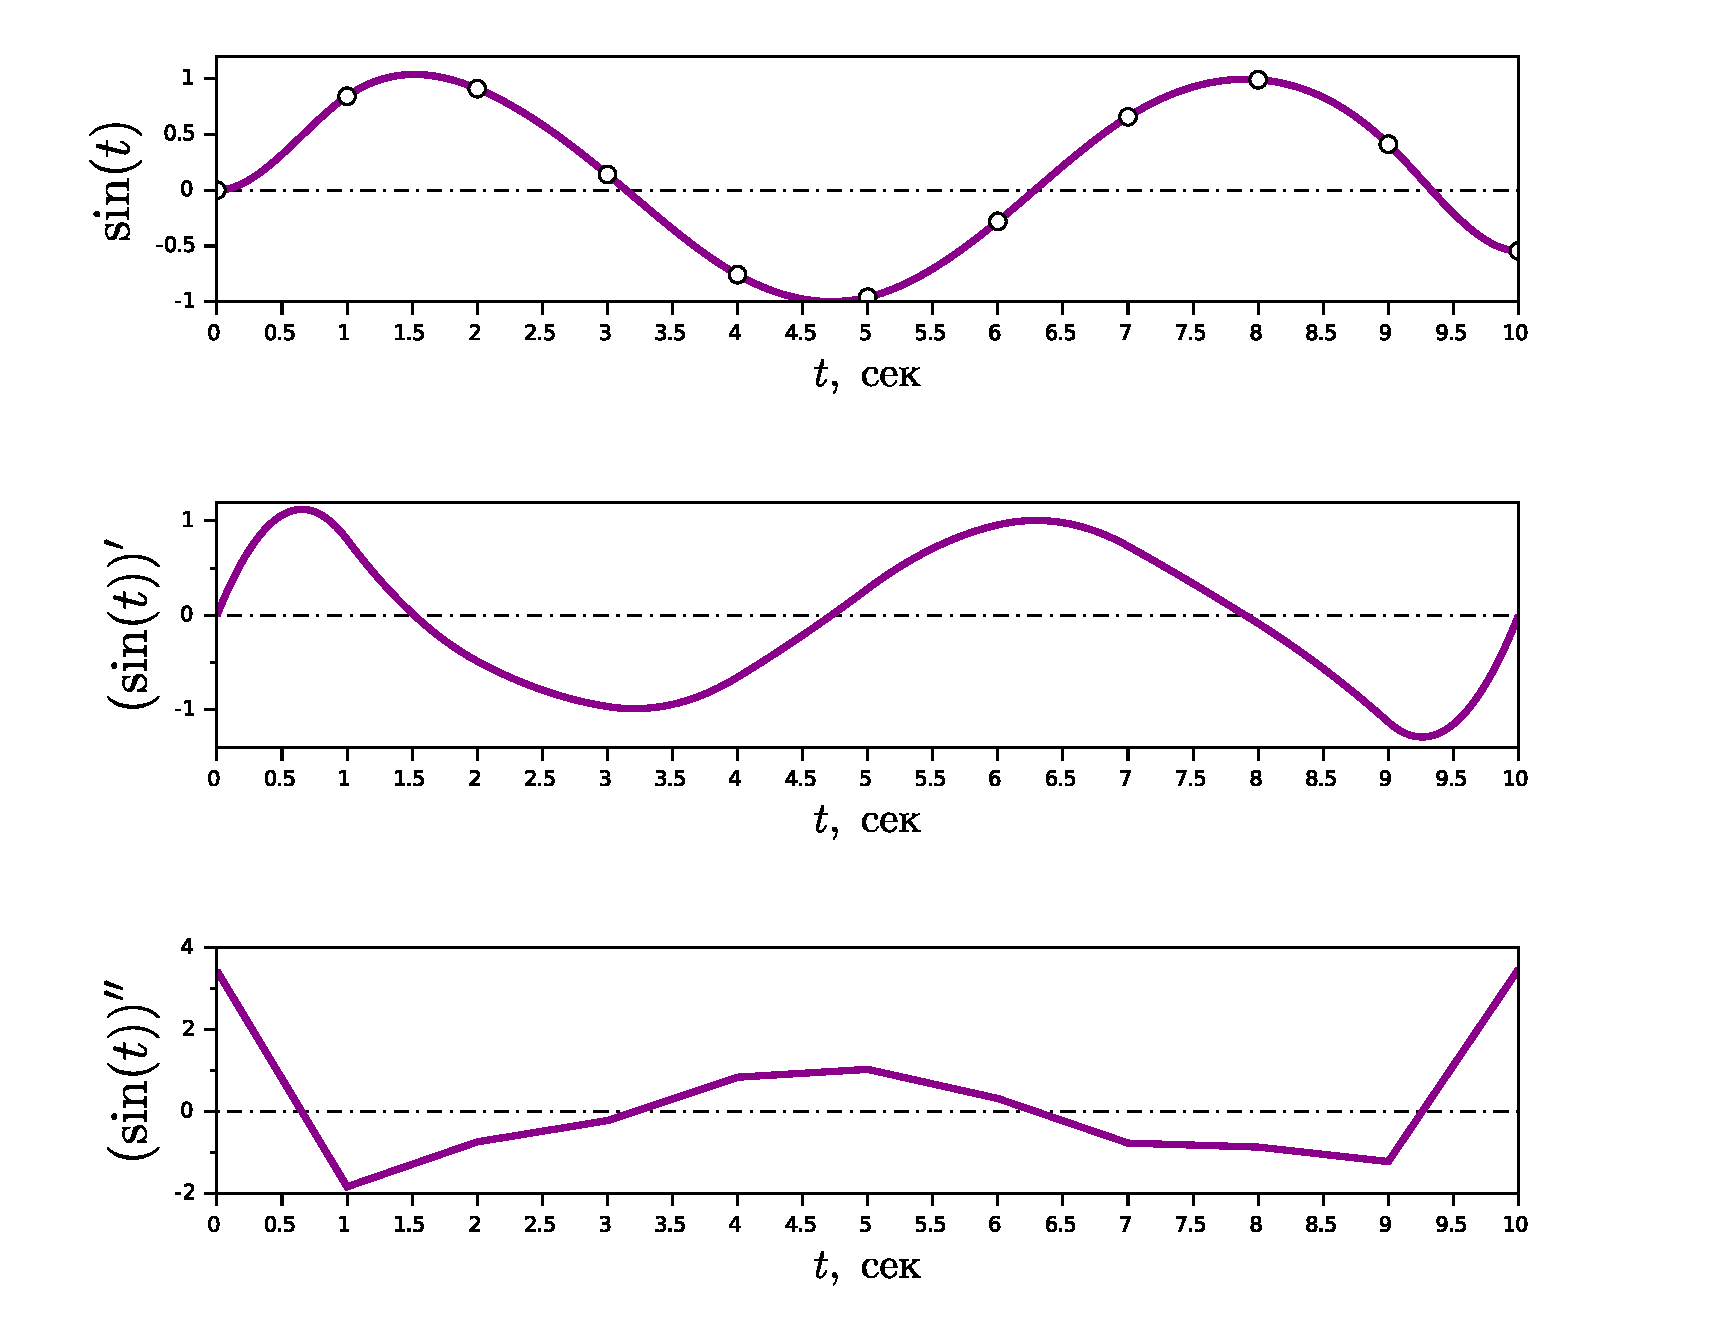
\includegraphics[width=\textwidth]{cubic_splines_examples.pdf}
	\vspace{0.5cm}
	\caption{Пример результата интерполяции набора из одиннадцати точек функции $\sin(t)$}
	\label{img:cubic_splines_method_test}
\end{figure}

Планирование траектории должно осуществляться перед началом работы. При реализации описаного метода может случиться так, что скорости и ускорения некоторых из компонентов векторов обобщенных координат будут превышать допустимые значения скоростей и ускорения, которые могут развить приводы манипулятора. Один и способов борьбы с этим~--- увеличить время прохождения траектории на участке, на котором ограничение нарушено.


%Далее, с помощью рекуррентных соотношений~\eqref{spline_equations}, \eqref{ck}, \eqref{dk} можно найти все коэффициенты $ c_k $ и $ d_k $, $ k = \overline{1,2,\dots,n} $, если принять последние соотношения в качестве начальных условий, после чего, вычислисть $ x_k $, $ k=\overline{n-1, n-2, \dots, 1} $.

%%%%%%%%%%%%%%%%%%%%%%%%%%%%%%%%%%%%%%%%%%%%%
%%%%%%%%%%%%%%%%%%%%%%%%%%%%%%%%%%%%%%%%%%%%%
%%%%%%%%%%%%%%%%%%%%%%%%%%%%%%%%%%%%%%%%%%%%%
\vspace{0.5cm}
\subsection{Планирование траектории в пространстве координат схвата}

Планирование траектории в пространстве координат схвата включает в себя два этапа: на первом этапе планируется траектория относительно базовой СК робота, на втором этапе~--- полученная траектория переводится в пространство обобщенных координат робота и трансформируется в рассмотренную выше задачу.

\begin{figure}[h!]
	\centering\includegraphics[width=1\textwidth]{ipe/trajectory_planning.pdf}
	\vspace{0.5cm}
	\caption{Планирование траекторий на конвейерах: слева~--- вращающийся стол; справа~--- линейный конвейер}
	\label{img:trajectory_planning}
\end{figure}

Для планирования траектории захвата движущегося по конвейеру объекта, получим аналитические выражения для геометрического пути следования этого объекта. 
Дальнейшие рассуждения и обозначения наглядно представлены на рисунке~\ref{img:trajectory_planning}.

Необходимо представить траекторию, как зависимость
\begin{equation}
	T = T(t),
\end{equation}
которая удовлетворяет требованиям плавного разгона и торможения, тогда
\begin{equation}\label{Tt}
	T(t) = T_0 \cdot A(\overrightarrow{n}, \delta(t), \rho(t)),
\end{equation}
где $ A(t) $ матрица однородных преобразований между точкой траектории и вектором обобщенных координат:
\begin{equation}
	A(t) = 
	\begin{bmatrix}
	R(t) & \mathbf{\rho}(t)\\
	000&1
	\end{bmatrix}\!.
\end{equation}

Заметим, что в соответствии с рисунком~\ref{img:trajectory_planning} и~\eqref{Tt}:
\begin{equation}
	T(t_0) =T_0, \quad T(t_0 + \tau) = T_0 \cdot T_f^{-1},
\end{equation}
\begin{equation}
	R(t_0) = E, \quad R(t_0+\tau) = R_0 \cdot R_f.
\end{equation}
\begin{equation}
	\rho(t_0) = 0, \quad \rho(t_0 + \tau) = R^T_0 (r_f - r_0),
\end{equation}
где $ r_0 $ и $ r_f $~--векторы переноса составленные из первых трех компонент векторов~$ \mathbf{p}_0 $ и~$ \mathbf{p}_f $.

Найдем вектор $ \overrightarrow{n} $, вокруг которого осуществляется поворот из следующих выражений:
\begin{equation}
	\delta(t_0 + \tau) = \arccos{\cfrac{r_{11} + r_{22} + r_{33} - 1}{2}},
\end{equation}
\begin{equation}
	\mathbf{n} = \cfrac{1}{2 \sin{\delta}} 
	\cdot
	\begin{bmatrix}
		r_{32} - r_{23} \\
		r_{13} - r_{31} \\
		r_{21} - r_{12}
	\end{bmatrix}\!,
\end{equation}
где $ r_{ij} $~--- элементы матрицы $ R(t_0 + \tau) $.

Окончательно, матрица поворота рассчитывается из выражения:
\begin{equation}\label{Rt}
	R(t) = \cos \delta(t) \cdot E + (1 - \cos \delta(t)) \cdot \mathbf{n} \cdot \mathbf{n}^T + \sin \delta(t) \cdot \Omega_n,
\end{equation}
где $ \Omega_n $~--- кососимметрическая матрица для вектора $ \mathbf{n} $.

Функции $ \rho(r) $ и $ \delta(t) $ выбираются исходя из условия обеспечения плавности разгона и торможения.

Для случая конвейера, представленного вращающимся столом, объект покоящийся на столе описывает окружность, закон движения по которой в плоскости параллельной плоскости OXY:
\begin{equation}
	\begin{cases}
		x(t) = R_c \cos{\theta(t)}\\
		y(t) = R_c \sin{\theta(t)} \\
		z(t) = const
	\end{cases}\!\!\!\!\!\!\!\!,
\end{equation}
где $ R_c $~--- радиус окружности, описываемой объектом при вращении стола, $ \theta(t) $~--- поворот стола.

Тогда, учитывая, что закон движения схвата манипулятора должен в точности повторять движение подвижного объекта, параметризуем закон движения схвата параметром поворота вращающегося стола $\theta = \theta(t)$, получим:
\begin{equation}
	\mathbf{p} = \mathbf{p}(\theta) = 
	\begin{bmatrix}
		R_c \cos{\theta}\\
		R_c \sin{\theta} \\
		z \\
		1
	\end{bmatrix}\!\!,
	\quad
	\theta \in [\theta_0,\,\,\theta_f].
\end{equation}

%%% the curve is regular
При этом нужно, чтобы выполнялось условие непрерывности траектории
\begin{equation}
	\dot{\mathbf{p}} = \cfrac{d \mathbf{p}}{d \theta} \ne 0,
	\quad
	\forall{\theta} \in [\theta_0,\,\,\theta_f].
\end{equation}

Траектория ориентации схвата определяется выражением~\eqref{Rt}

В этом разделе были проанализированы конфигурация и необходимая ориентация схвата в рабочем пространстве манипулятора робота KUKA Yobot. После этого были решены задачи планирования траекторий для перевода манипулятора из точки в точку, для обхода последовательности точек и для задания закона движения в пространстве координат схвата.

%\subsection{Геометрия рабочего пространства манипулятора}
%\subsubsection{Конфигурация рабочего пространства}
%\subsubsection{Анализ ориентации схвата в рабочем пространстве}

%\subsection{Кинематические свойства манипулятора}
%\subsubsection{Распределение допустимых скоростей}
%\subsubsection{Оценка мобильности и приемистости манипулятора}

\newpage



